%% from aastex61.cls with a few tweaks to allow for the unique format required.
\documentclass{rnaastex}

\begin{document}

\title{Radio line broadening from a spectral response function}

%% Note that the corresponding author command and emails has to come
%% before everything else. Also place all the emails in the \email
%% command instead of using multiple \email calls.
\correspondingauthor{Eric Koch}
\email{ekoch@ualberta.ca}
\author[0000-0001-9605-780X]{Eric Koch}
\author[0000-0002-5204-2259]{Erik Rosolowsky}
\affiliation{University of Alberta, Department of Physics 4-183 CCIS, Edmonton AB T6G 2E1, Canada}
\author[0000-0002-2545-1700]{Adam K. Leroy}
\affiliation{The Ohio State University, Department of Astronomy, 140 West 18th Avenue, Columbus, OH 43210, USA}


%% Note that RNAAS manuscripts DO NOT have abstracts.
%% See the online documentation for the full list of available subject
%% keywords and the rules for their use.
\keywords{methods: observational}

%% Start the main body of the article. If no sections in the
%% research note leave the \section call blank to make the title.

\section{}

All spectral-line observations are broadened by the spectrometer response function, but analyses of radio data often assume independent channels.  Typical observing strategies resolve lines with $\sim3-5$ channels per full-width-half-max, which bias line width measurements that assume independent channels.  Here, we compare methods for inferring line width and how the spectral response affects them.

We consider a noiseless Gaussian with dispersion $\sigma$ as the simplest model.  Using an ideal spectrometer, each channel is independent and the Gaussian is smoothed with a top-hat kernel one channel in width ($\Delta v$).  This smoothing lower the amplitude and increases $\sigma$ in the observed spectrum, and becomes more extreme as $\Delta v \rightarrow \sigma$.

Real spectrometers have more complex spectral responses than a top-hat.  Fourier transform spectrometers typically have a sinc-like frequency response.  Apodizing kernels, including the Hann kernel, reduce the ``ringing'' from sinc but correlate nearby channels\footnote{\url{https://safe.nrao.edu/wiki/pub/Main/ALMAWindowFunctions/Note_on_Spectral_Response.pdf}}.  Instruments with well-characterized response functions can be modelled in observed spectra \citep{rosolowsky2008}.  Without this information, a three-element Hann-like kernel ($[k, 1 - 2k, k]$ with channel-coupling $k$) can approximate the nearest-neighbour correlations \citep{leroy2016}.

The top row in Figure \ref{fig:width_recovery_comparison} shows a Gaussian averaged over independent channels and convolved with a Hann-like kernel with $\Delta v=\sigma$ ($k=0.11$).  The two panels show how line broadening depends on whether the line is positioned in the centre (minimal broadening) or edge (maximal broadening) of a channel.  As a source property, the positioning cannot be assumed beforehand.

% To recover the line properties, the spectral response can be included in the model for the observed spectrum.
The spectral response can be forward-modeled when fitting the observed spectrum by convolving with a Hann-like kernel.  Forward-modelling the spectral response is common-practice in many fields \citep[e.g.,][]{martin2015}, but is seldom used in radio studies.  Without noise, this model correctly recovers the line properties.

% While forward-modelling accounts for the spectral response, the spectrum must be fit, which requires knowing a correct model and may be affected by noise.
Forward-modelling requires fitting the spectrum, which can be difficult with noisy data. Instead, many studies use approximations to estimate the line width:
% We compare forward-model fitting with:
\begin{enumerate}
    \item {\bf Fit to Gaussian} without forward-modelling.
    \item {\bf Moment 2}: $\sigma_{\rm Mom2}=\sqrt{\sum_i T_i (v_i - v_0)^2 / \sum_i T_i}$ where $T_i$ is the value at $v_i$ and $v_0$ is the centroid.
    \item {\bf Equivalent width}: $\sigma_{\rm equiv} = T_{\rm peak} / \sqrt{2\pi} \Sigma$ where $T_{\rm peak}$ is the measured amplitude and $\Sigma= \sum_i T_i \Delta v$ \citep{heyer2001,leroy2016,sun2018}.
    \item {\bf Half-width-half-max (HWHM)} estimated from where the observed spectrum is half the peak \citep{stilp2013a,stilp2013b,koch2018}.
\end{enumerate}

Many studies correct the measured line width by subtracting in quadrature a factor for top-hat kernel broadening, namely $\Delta v / \sqrt{2\pi}$ \citep{cprops}.  To account for channel correlations, \citet{leroy2016} extended this correction factor with an empirical calibration relating channel correlations to a Hann-like kernel:
% ($k\approx 0.0 + 0.47r - 0.23r^2 - 0.16r^3 + 0.43 r^4$).
\begin{equation}
    \label{eq:leroy16_corrfact}
    \sigma_{\rm chan} \approx \frac{\Delta v}{\sqrt{2\pi}} \left( 1.0 + 1.18k + 10.4k^2 \right).
\end{equation}
As $k\rightarrow0$, the equation reduces to $\Delta v / \sqrt{2\pi}$.  We adopt $k=0.11$ for our example \citep{sun2018}.

We generate model spectra varying the sampling $\Delta v / \sigma$ and calculating the line width from each method, with and without subtracting Eq. \ref{eq:leroy16_corrfact}, for independent channels (top-hat) and correlated channels. The bottom four panels in Figure \ref{fig:width_recovery_comparison} show the measured line widths.

When the line is centered on a channel (first column), the line width methods are comparable and convolving with a Hann-like kernel only broadens the spectra.  Line widths are over-corrected with Eq. \ref{eq:leroy16_corrfact} when $k=0$, but are within $<5\%$ for correlated channels when $\sigma/\Delta v \geq 1$.

There are deviations between the methods when the line is centered on the channel edge (second column). The Gaussian fit and second moment are biased similarly to when the peak is centered on a channel.  The equivalent width and HWHM are biased to larger values than the latter methods because they depend on the amplitude of the profile, which is underestimated more than in the channel-centre case.
% Eq. \ref{eq:leroy16_corrfact} {\it underestimates} the line broadening in this case. Methods that leverage information across many channels are preferable over those that use only the line core when $\sigma / \Delta v < 2$.

Our results show:
\begin{enumerate}
    \item Line width measurements depend on the spectral response and must be modelled correctly. In our example, a Hann-like kernel increased measured line widths by $\sim10\%$ compared to the top-hat kernel.
    \item The independent channel correction $\Delta v / \sqrt{2\pi}$ is not the line width contribution for a top-hat kernel and should not be used.
    \item To recover accurate line widths within $<5\%$ for correlated channels, $\sigma / \Delta v \geq 2$ is needed for fitting a Gaussian and the second moment, while $\sigma / \Delta v \geq 4$ is needed for the equivalent width and HWHM.
    % Broadening from the spectral response is negligible above these limits.
    Where possible, we recommend that observational setups sample $\sigma / \Delta v > 2$.
    \item Fitting analytical models to observed data should account for the spectral response via forward-modelling when $\sigma / \Delta v \leq 2$.
    \item Line width methods that use information over multiple channels (fitting, second moment) are preferable over those that use the line core (equivalent width, HWHM). These latter methods should be treated with caution when $\sigma / \Delta v <4$.
\end{enumerate}

These recommendations are only for {\it high signal-to-noise, Gaussian spectra}. Noise or multi-component spectra will change the biases for these methods and can be explored for individual data sets.
% We also note that these methods will break down when the Gaussian assumption is invalid \citep{koch2018}.

Code is available at: \url{https://doi.org/10.5281/zenodo.1491796}.

% The examples in Figure \ref{fig:width_recovery_comparison} do not include noise in the spectra.  We test the forward-modelling model in the presence of noise drawn to give a peak signal-to-noise of 5 in the spectrum.  The noisy spectrum is then convolved with the response function used above to correlate the noise.  Drawing 1000 iterations of noise, we find that the fitted parameters are not biased by line broadening.  However, the Levenberg-Marquadt algorithm used for the fitting assumes that the noise is uncorrelated.  We test whether breaking this assumption significantly underestimates the parameter uncertainties from the covariance matrix by calculating the fraction of iterations that the true parameter value lies within the $1\mbox{-}\sigma$ uncertainty range from the fit.  We find that true values are within the uncertainty range in $\sim70\%$ of the iterations, similar to the expected $68.2\%$ for the $1\mbox{-}\sigma$ range for a Gaussian distribution.  The lack of modelling for correlated errors should not significantly change the uncertainties.  The correlated noise may become more important if the spectral response function correlates channels beyond their nearest neighbours.  In that case, a Gaussian process can be used to model the correlated uncertainties XXX rasmussen and michaels XXX.


\begin{figure*}
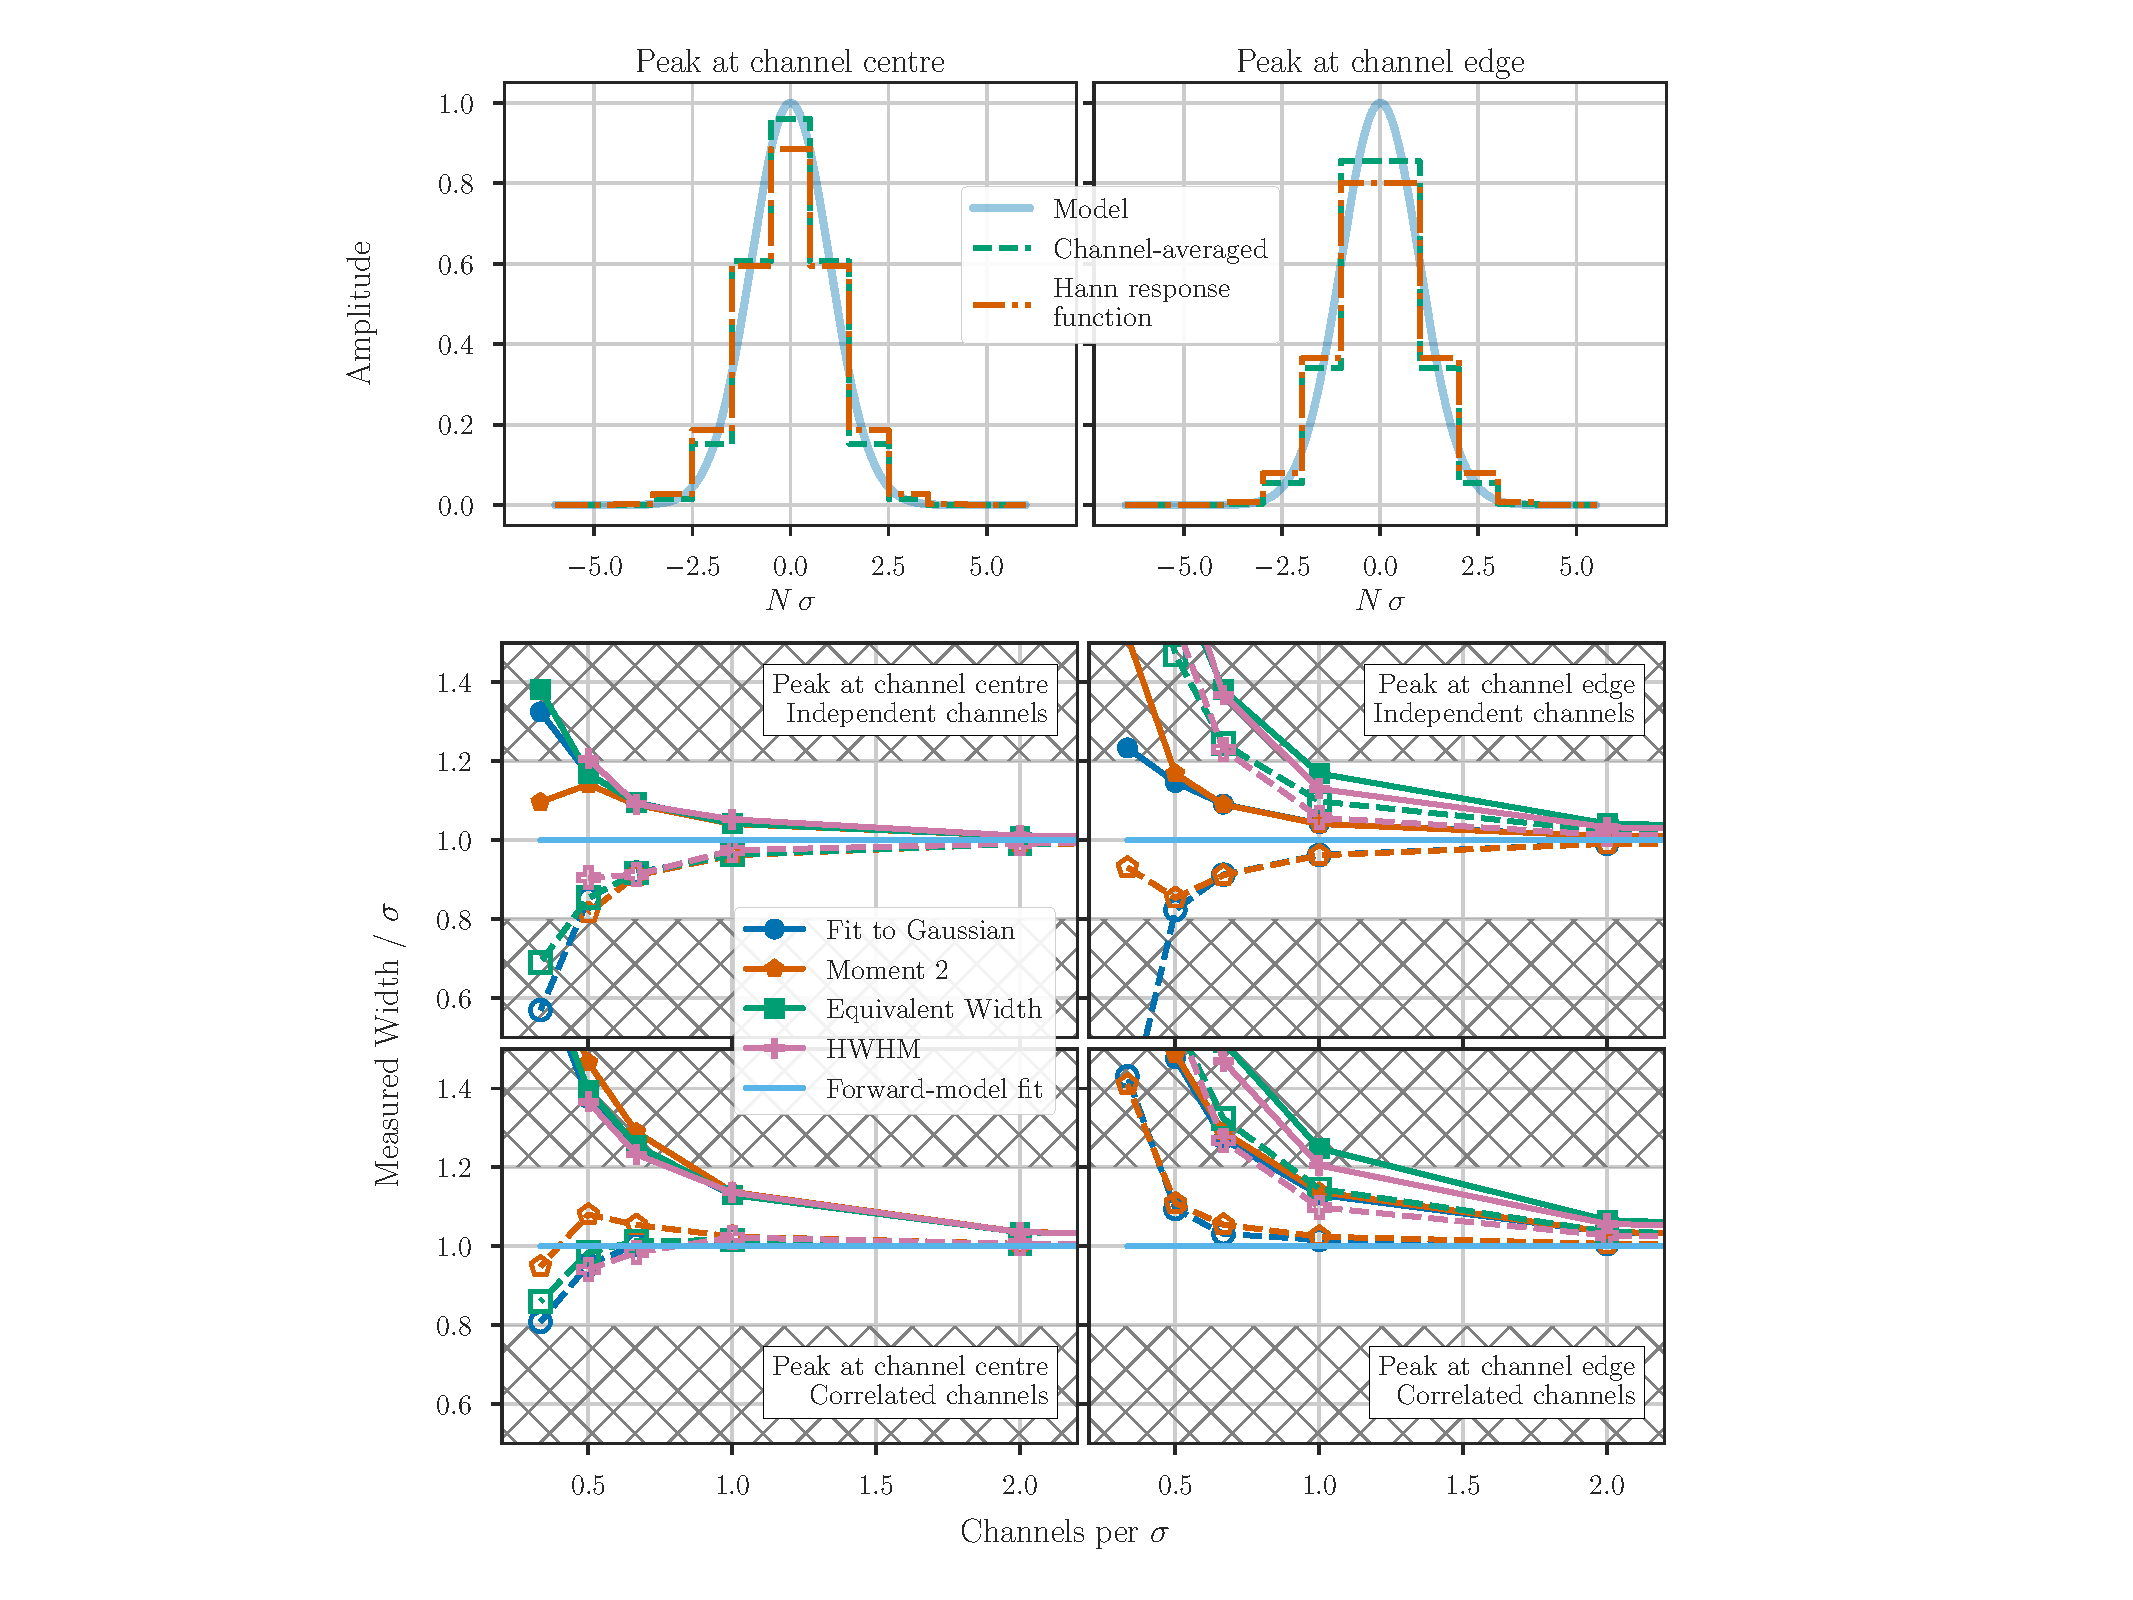
\includegraphics[width=\textwidth]{combined_figure}
\caption{\label{fig:width_recovery_comparison} Top row: Gaussian (blue-solid) sampled with $\Delta v = \sigma$ (dashed) and convolved with a Hann-like kernel (dot-dashed) with the peak at the channel centre (left) and edge (right). Bottom rows: Percent deviation in the measured line widths with increasing $\Delta v / \sigma$ (solid lines). The middle row shows spectra with independent channels and the bottom row is convolved with a Hann-like kernel ($k=0.11$). Dashed lines are corrected with Eq. \ref{eq:leroy16_corrfact}.}
\end{figure*}

\acknowledgments

EWR acknowledges support from the Natural Sciences and Engineering Research Council of Canada (RGPIN-2017-03987). AKL is partially supported by the National Science Foundation under Grants No. 1615105, 1615109, and 1653300.

\software{astropy \citep{astropy}}

\begin{thebibliography}{}

\bibitem[Astropy Collaboration et al.(2018)]{astropy} Astropy Collaboration, Price-Whelan, A.~M., Sip{\'{o}}cz, B.~M., et al.\ 2018, AJ, 156, 123.

\bibitem[Heyer et al.(2001)]{heyer2001} Heyer, M.~H., Carpenter, J.~M., \& Snell, R.~L.\ 2001, ApJ, 551, 852.

\bibitem[Koch et al.(2018)]{koch2018} Koch, E.~W., Rosolowsky, E.~W., Lockman, F.~J., et al.\ 2018, MNRAS, 479, 2505.

\bibitem[Leroy et al.(2016)]{leroy2016} Leroy, A.~K., Hughes, A., Schruba, A., et al.\ 2016, ApJ, 831, 16.

\bibitem[Martin et al.(2015)]{martin2015} Martin, T., Drissen, L., \& Joncas, G.\ 2015, ADASS XXIV, 327.

\bibitem[Rosolowsky, \& Leroy(2006)]{cprops} Rosolowsky, E., \& Leroy, A.\ 2006, PASP, 118, 590.

\bibitem[Rosolowsky et al.(2008)]{rosolowsky2008} Rosolowsky, E.~W., Pineda, J.~E., Foster, J.~B., et al.\ 2008, ApJS, 175, 509.

\bibitem[Stilp et al.(2013a)]{stilp2013a} Stilp, A.~M., Dalcanton, J.~J., Warren, S.~R., et al.\ 2013, ApJ, 765, 136.

\bibitem[Stilp et al.(2013b)]{stilp2013b} Stilp, A.~M., Dalcanton, J.~J., Skillman, E., et al.\ 2013, ApJ, 773, 88.

\bibitem[Sun et al.(2018)]{sun2018} Sun, J., Leroy, A.~K., Schruba, A., et al.\ 2018, ApJ, 860, 172.


\end{thebibliography}

\end{document}
